% Chapter1.tex

\section{BP算法推导}

反向传播算法使用梯度下降策略对神经网络参数进行调整。以全连接神经网络为例,如\reffig{fig:nn-module-complete},该网络有三层:

\begin{enumerate}
\item 含有$d$个神经元的输入层
\item 含有$q$个神经元的隐层
\item 含有$l$个神经元的输出层
\end{enumerate}

假设网络的激活函数都是Sigmoid函数,即$f(x)=\frac{1}{1+e^{-x}}$,每个神经元接受的输入如\reffig{fig:nn-module-complete}所示,

\begin{figure}[tbph]
\centering
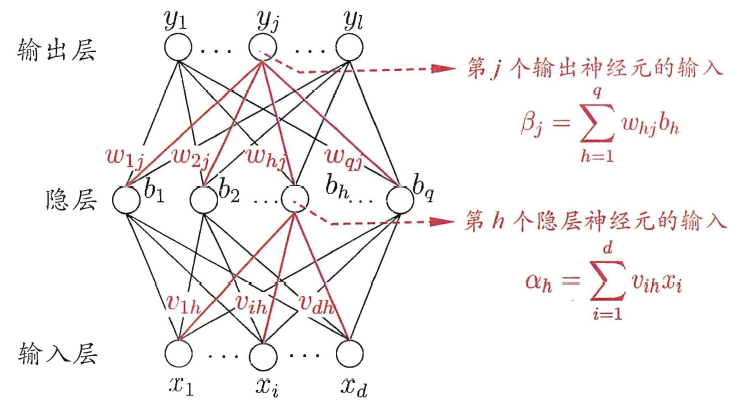
\includegraphics[width=0.75\linewidth]{.asserts/nn-module-complete}
\caption{含有单层隐含层的三层神经网络}
\label{fig:nn-module-complete}
\end{figure}

定义误差函数为$E=\frac{\sum_{i=1}^{l}{(\hat{y_i} - y_i)^2}}{2}$,即均方误差函数。以隐层到输出层的参数调整为例。

\subsection{权重调整}

权重$w_{ij}$的调整方式如\refeq{eq:update-w}。

\begin{equation}\label{eq:update-w}
\begin{aligned}
\Delta w_{ij} &= -\eta \frac{\partial E}{\partial w_{ij}} \\
&= -\eta \frac{\partial E}{\partial \hat{y_j}} \frac{\partial \hat{y_j}}{\partial \hat{\beta_j}} \frac{\partial \hat{\beta_j}}{\partial w_{ij}}
\end{aligned}
\end{equation}

由于$\frac{\partial E}{\partial \hat{y_j}} = \hat{y_j} - y_j$,Sigmoid函数满足$f\prime(x)=f(x)(1-f(x))$,$\frac{\partial \hat{\beta_j}}{\partial w_{ij}}=b_i$。因此\refeq{eq:update-w}可以变换为如\refeq{eq:update-w-convert}形式。

\begin{equation}\label{eq:update-w-convert}
\begin{aligned}
\Delta w_{ij} &= -\eta (\hat{y_j} - y_j) (\hat{y_j}(1-\hat{y_j})) (b_i) \\
&= -\eta b_i \hat{y_j} (\hat{y_j} - y_j) (1 - \hat{y_j})
\end{aligned}
\end{equation}

\subsection{阈值调整}

类似于权重调整,也对$E$求阈值$\theta$的导数。

\begin{equation}\label{eq:update-theta}
\begin{aligned}
\Delta \theta_{j} &= -\eta \frac{\partial E}{\partial \hat{y_j}} \frac{\partial \hat{y_j}}{\partial \theta_j}
\end{aligned}
\end{equation}

由于Sigmoid函数满足$f\prime(x)=f(x)(1-f(x))$,因此\refeq{eq:update-theta}可以变换为如\refeq{eq:update-theta-convert}形式。

\begin{equation}\label{eq:update-theta-convert}
\begin{aligned}
\Delta \theta_{j} &= -\eta (\hat{y_j} - y_j) (-1)(\hat{y_j}(1-\hat{y_j}))\\
&= \eta \hat{y_j} (\hat{y_j} - y_j) (1-\hat{y_j})
\end{aligned}
\end{equation}

每次训练后,朝误差减少的方向调整参数。其中$\eta$是学习率。